\chapter{نمونه‌ها و ابزار‌ها}\label{chp:chap3}
\thispagestyle{empty}
% \rhead{\leftmark}
%================================================================================
\section{مقدمه ای بر استفاده از بسته‌ها}\label{seq3.1}
در این بخش به طور خلاصه بیان می‌کنیم که چطور می‌توان شکل وارد نمود و یا نمونه کد و جدول و ... را به فایل مطلوبمان اضافه کرد. همانطور که قبلا نیز اشاره شد در لاتک با استفاده از بسته‌های مختلف می توان از ابزار‌هایی استفاده کرد که با آن اشکال، جداول، نمودارها و به طور کلی اجزای یک سند را شکل داد. این ابزارها که به صورت بسته‌های لاتک فراخوانی می‌شوند و از ابزار‌ها آنها می توان استفاده کرد. در زیر برخی از بسته‌های لاتک و امکاناتی را که در اختیار قرار می دهند آورده‌ایم.در زمان نوشتن این گفتار تعداد بسته‌های رسمی لاتک بیش از ۵۴۰۰ و بسته‌های غیر رسمی بیش از ۲۵۰۰ عدد است.
% \begin{table}
% % \begin{center}
\begin{latin}
%  \begin{tabular}{|m{0.2\linewidth}|m{0.8\linewidth}|}
\begin{longtable}{| p{.20\textwidth} | p{.80\textwidth} |}
 \hline
  amsmath &It contains the advanced math extensions for LaTeX. The complete documentation should be in your LaTeX distribution; the file is called amsdoc, and can be dvi or pdf. For more information, see the chapter about Mathematics. Successed by mathtools package described below.\\\hline
amssymb&It adds new symbols in to be used in math mode.\\\hline
amsthm&It introduces the proof environment and the {\color{green}\textbackslash{theoremstyle}} command. For more information see the Theorems section.\\\hline
array&It extends the possibility of LaTeX to handle tables, fixing some bugs and adding new features. Using it, you can create very complicated and customized tables. For more information, see the Tables section.\\\hline
babel&It provides the internationalization of LaTeX. It has to be loaded in any document, and you have to give as an option the main language you are going to use in the document. For more information see the Internationalization section.\\\hline
biblatex&Advanced bibliography handling. It is the package to use for writing a thesis.\\\hline
bm&Allows use of bold greek letters in math mode using the{\color{green} \textbackslash{bm}\{\dots\}} command. This supersedes the amsbsy package.\\\hline
booktabs &provides ex­tra com­mands as well as be­hind-the-scenes op­ti­mi­sa­tion for producing tables. Guide­lines are given as to what con­sti­tutes a good ta­ble in the package documentation.\\\hline
boxedminipage &It introduces the boxedminipage environment, that works exactly like minipage but adds a frame around it.\\\hline
caption &Allows customization of appearance and placement of captions for figures, tables, etc.\\\hline
% cancel &Provides commands for striking out mathematical expressions. The syntax is
% \begin{latin}
% \begin{lstlisting}[style=Tex]
% \cancel{x} or \cancelto{0}{x}
% \end{lstlisting}
% \end{latin}
% \\\hline
% chemmacros &Part of a bundle to typeset chemistry easily and consistent.\\\hline
% changepage &To easily change the margins of pages. The syntax is
% \begin{latin}
% \begin{lstlisting}[style=Tex]
% \changepage{textheight}{textwidth}%
%   {evensidemargin}{oddsidemargin}%
%   {columnsep}{topmargin}%
%   {headheight}{headsep}%
%   {footskip}
% \end{lstlisting}
% \end{latin}
% All the arguments can be both positive and negative numbers; they will be added (keeping the sign) to the relative variable.\\\hline
cleveref &En­hances LaTeX's cross-ref­er­enc­ing fea­tures, al­low­ing the for­mat of ref­er­ences to be de­ter­mined au­to­mat­i­cally ac­cord­ing to
the type of ref­er­ence.\\\hline
dcolumn &The package defines a new "D" column format in tab­u­lar en­vi­ron­ments for aligning the numbers in columns on the decimal point.\\\hline
enumitem &Adds support for arbitrarily-deep nested lists (useful for outlines). See List Structures.\\\hline
epstopdf &Provides and option to convert EPS images to PDF and include them with \textbackslash{includegraphics}\{\}.\\\hline
esint &Adds additional integral symbols, for integrals over squares, clockwise integrals over sets, etc.\\\hline
eucal &Other mathematical symbols.\\\hline
fancyhdr &To change header and footer of any page of the document. It is described in the Page Layout section.\\\hline
float &Im­proves the in­ter­face for defin­ing float­ing ob­jects such as fig­ures and ta­bles, introduces new floating objects types (boxed, ruled, plaintop) and provides an ability to define custom ones.\\\hline
fontenc &To choose the font encoding of the output text. You might need it if you are writing documents in a language other than English. Check in the Fonts section.\\\hline
gensymb &Pro­vides generic com­mands \textbackslash{de­gree}, \textbackslash{cel­sius}, \textbackslash{pert­hou­sand}, \textbackslash{mi­cro} and \textbackslash{ohm} which work both in text and maths mode.\\\hline
geometry &For easy management of document margins and the document page size. See Page Layout.\\\hline
glossaries &For creation of glossaries and list of acronyms. For more information, see the relevant chapter.\\\hline
graphicx &Allows you to insert graphic files within a document.\\\hline
grffile &Improves the file name pro­cess­ing of graphic/graphicx pack­ages to sup­port a larger range of file names (spaces, multiple dots, etc.).\\\hline
hyperref &It gives LaTeX the possibility to manage links within the document or to any URL when you compile in PDF. For more information, see the relevant section.\\\hline
indentfirst &Once loaded, the beginning of any chapter/section is indented by the usual paragraph indentation.\\\hline
inputenc &To choose the encoding of the input text. You might need it if you are writing documents in a language other than English. Check in the Special Characters section.\\\hline
latexsym &Other mathematical symbols.\\\hline
listings &To insert programming code within the document. Many languages are supported and the output can be customized. For more information, see the Source Code Listings.\\\hline
longtable &Al­lows you to write ta­bles that con­tinue to the next page. You can also define a header and a footer which will be shown on every page the table occupies, for example cont. from last page.\\\hline
mathptmx &Sets the default font of the entire document (including math formulae) to Times New Roman, which is a more familiar font, and useful in saving space when fighting against page limits.\\\hline
mathrsfs &Other mathematical symbols.\\\hline
mathtools &Successor of amsmath, some additional functionality, some bugs fixed.\\\hline
mhchem &allows you to easily type chemical species and equations. It automatically formats chemical species so you don't have to use subscript commands. It also Allows you to draw chemical formulas.\\\hline
microtype &It provides an improvement to LaTeX's default ty­po­graphic ex­ten­sions, improvements in such areas as char­ac­ter pro­tru­sion and font ex­pan­sion, in­ter­word spac­ing and ad­di­tional kern­ing, and hy­phen­at­able letter-spacing\\\hline
multicol &provides the mul­ti­cols environment which typesets text into multiple columns.\\\hline
natbib &Gives additional citation options and styles. Often used for journal submission.\\\hline
pdfpages &This package simplifies the insertion of external multi-page PDF or PS documents.\\\hline
rotating &It lets you rotate any kind of object. It is particularly useful for rotating tables. For more information, see the relevant section.\\\hline
setspace &Lets you change line spacing, e.g. provides the \doublespacing command for making double spaced documents. For more information, see the relevant section.\\\hline
showkeys &A useful package related to referencing. If you wish to reference an image or formula, you have to give it a name using \textbackslash{label}\{\dots\} and then you can recall it using \textbackslash{ref}\{\dots\}. When you compile the document these will be replaced only with numbers, and you can't know which label you had used unless you take a look at the source. If you have loaded the showkeys package, you will see the label just next or above the relevant number in the compiled version. An example of a reference to a section is Latex showkeys example.png. This way you can easily keep track of the labels you add or use, simply looking at the preview (both dvi or pdf). Just before the final version, remove it.\\\hline
showidx &It prints out all index entries in the left margin of the text. This is quite useful for proofreading a document and verifying the index. For more information, see the Indexing section.\\\hline
subfiles &The "root" and "child" document can be compiled at the same time without making changes to the "child" document. For more information, see the Modular Documents section.\\\hline
subcaption &It allows to define multiple floats (figures, tables) within one environment giving individual captions and labels in the form 1a, 1b.\\\hline
% syntonly &If you add the following code in your preamble:
% \begin{latin}
% \begin{lstlisting}[style=Tex]
% \usepackage{syntonly}
% \syntaxonly
% \end{lstlisting}
% \end{latin}
% LaTeX skims through your document only checking for proper syntax and usage of the commands, but doesn’t produce any (DVI or PDF) output. As LaTeX runs faster in this mode you may save yourself valuable time. If you want to get the output, you can simply comment out the second line.\\\hline
textcomp &Provides extra symbols, e.g. arrows like \textbackslash{textrightarrow}, various currencies (\textbackslash{texteuro},...), things like \textbackslash{textcelsius} and many others.\\\hline
theorem &You can change the style of newly defined theorems. For more information see the Theorems section.\\\hline
todonotes &Lets you insert notes of stuff to do with the syntax \textbackslash{todo}\{Add details.\}.\\\hline
siunitx &Helps you typeset of SI-units correctly. For example \textbackslash{SI}\{12\}\{\textbackslash{mega}\textbackslash{hertz}\}. Automatically handles the correct spacing between the number and the unit. Note that even non-SI-units are set, like dB, rad, ...\\\hline
ulem &It allows to underline text (either with straight or wavy line). Few examples of usage are added to the Fonts chapter.\\\hline
url &It defines the \textbackslash{url}\{\dots\} command. URLs often contain special character such as \'\_\' and \'\&\', in order to write them you should escape them inserting a backslash, but if you write them as an argument of \textbackslash{url}\{\dots\}, you don't need to escape any special character and it will take care of proper formatting for you. If you are using hyperref, you don't need to load url because it already provides the \textbackslash{url}\{\dots\} command.\\\hline
verbatim &It improves the verbatim environment, fixing some bugs. Moreover, it provides the comment environment, that lets you add multiple-line comments or easily comment out big parts of the code.\\\hline
xcolor &It adds support for colored text. For more information, see the relevant section.\\\hline
xypic &It is used to create trees, graphs, (commutative) diagrams, and similar things. See Xy-pic.\\\hline
% % \end{center}
\end{longtable}
%  \end{tabular}
\end{latin}
% \end{table}

\section{فرمولها}\label{seq:3.2}
فرمول‌نویسی و شماره گذاری فرمول‌ها در لاتک بسیار ساده است . کد زیر 
\begin{latin}
\begin{lstlisting}[style=Tex]
\begin{equation}\label{eq:1.2.2}
\bar{r}_{r\mathbf{R}}=\langle{\mathbf{R}n}|r|\mathbf{R}n\rangle
\end{equation}
\end{lstlisting}
\end{latin}
خروجی زیر را می دهد.
\begin{equation}\label{eq:1.2.2}
\bar{r}_{r\mathbf{R}}=\langle{\mathbf{R}n}|r|\mathbf{R}n\rangle
\end{equation}
همانطور که دیده می‌شود  برای نوشتن عبارات در فرمول‌ها از دستور زبان خاصی استفاده می شود که IDE ها معمولا این موارد را به صورت گرافیکی در اختیار قرار می دهند و افراد با استفاده از آنها به راحتی آنها را  در کد لاتک خود درج می کنند.  کلید 
\lr{\textbackslash{label\{eq:1.2.2\}}}
چاپ نمی‌شود و فقط برای ارجاع به فرمول است عبارت \lr{eq:1.2.2} یک عبارت اختیاری است که شما می توانید به دلخواه آن را تنظیم کنید و هر جایی که می‌خواهید  به فرمول فوق ارجاع دهید با استفاده از 
\lr{\textbackslash{ref\{eq:1.2.2\}}}
 می‌توانید این ارجاع را وارد کنید که در متن به شکل \ref{eq:1.2.2} چاپ می شود. مثلا می گوییم در فرمول \ref{eq:1.2.2} ما یک معادله گفتیم.
 
 فرمول‌ها می توانند چند خط باشند 
 \begin{latin}
\begin{lstlisting}[style=Tex]
 \begin{gather}
\psi _{n\mathbf{k}} ({\bf r}) = u_{n\mathbf{k}} ({\bf r})  \exp{(i\mathbf{k.r})} \\
 u_\mathbf{k}({\bf r})=u_\mathbf{k}({\bf r}+\mathbf{R})
\end{gather}
\end{lstlisting}
\end{latin}
که می شود
 \begin{gather}
\psi _{n\mathbf{k}} ({\bf r}) = u_{n\mathbf{k}} ({\bf r})  \exp{(i\mathbf{k.r})} \\
 u_\mathbf{k}({\bf r})=u_\mathbf{k}({\bf r}+\mathbf{R})
\end{gather}
ویا هم خط شده باشند
 \begin{latin}
\begin{lstlisting}[style=Tex]
\begin{align}\label{eq2}
w_n({\bf r}-\mathbf{R})=\left|\mathit{\mathbf{R}n}\right\rangle &=\frac {V}{(2\pi )^3}\int 
_{\mathit{BZ}}\mathit{d\mathbf{k}}\exp{(-\mathit{i\mathbf{k}.\mathbf{R}})}\left|\psi \right\rangle \\ 
&= \frac V{(2\pi )^3}\int 
_{\mathit{BZ}}\mathit{d\mathbf{k}}\exp{(-\mathit{i\mathbf{k}.\mathbf{R}})}u_{\mathit{n\mathbf{k}}}({\bf r})e^{\mathit{i\mathbf{k.r}}}\nonumber
\end{align}
\end{lstlisting}
\end{latin}
که می‌شود
\begin{align}\label{eq2}
w_n({\bf r}-\mathbf{R})=\left|\mathit{\mathbf{R}n}\right\rangle &=\frac {V}{(2\pi )^3}\int 
_{\mathit{BZ}}\mathit{d\mathbf{k}}\exp{(-\mathit{i\mathbf{k}.\mathbf{R}})}\left|\psi \right\rangle \\ 
&= \frac V{(2\pi )^3}\int 
_{\mathit{BZ}}\mathit{d\mathbf{k}}\exp{(-\mathit{i\mathbf{k}.\mathbf{R}})}u_{\mathit{n\mathbf{k}}}({\bf r})e^{\mathit{i\mathbf{k.r}}}\nonumber
\end{align}
که محل هم خط سازی را با علامت \lr{\&} مشخص می کنیم . گاهی نیاز است در فرمول ما شماره فرمول نداشته باشیم. برای این موارد از 
\lr{\textbackslash{nonumber}}

چنانچه بخواهیم عبارتی مانند $\epsilon$  یا  $ \bar{r}_{r\mathbf{R}}=\langle{\mathbf{R}n}|r|\mathbf{R}n\rangle$ که عباراتی ریاضی هستند در وسط متن بنویسیم آنها را  بین دو \$ قرار می دهیم. به عبارتی دیگر متن 
 \begin{latin}
\begin{lstlisting}[style=Tex]
 %*\rl{است }*) $ \bar{r}_{r\mathbf{R}}$   %*\rl{ این یک نمونه فرمول در وسط  متن }*)
\end{lstlisting}
\end{latin}
خروجی به شکل :
  این یک نمونه فرمول در وسط  متن  $ \bar{r}_{r\mathbf{R}}$ است.
  
ماتریس هم به شکل زیر نوشته می شود
 \begin{latin}
\begin{lstlisting}[style=Tex]
 \begin{equation}
  S= \begin{pmatrix}
      S_{cc} & S_{cv} \\
      S_{vc} & S_{vv}\\
      \end{pmatrix}
 \end{equation}
\end{lstlisting}
\end{latin}
که می شود
 \begin{equation}
  S=
 \begin{pmatrix}
 S_{cc} & S_{cv} \\
 S_{vc} & S_{vv}\\
 \end{pmatrix}
 \end{equation}
 
 نمونه‌ای از یک فرمول طولانی که در چند خط آمده  است به شکل زیر است.
  \begin{latin}
\begin{lstlisting}[style=Tex]
 \begin{align}
 \langle {\bf s}^{\prime}L^{\prime} | H | R{\bf s}L\rangle= & \langle {\bf s}^{\prime}L^{\prime}|-\frac{\Delta}{2} +\sum_{L_{1}} v_{{\bf s}^{\prime}L_1}(|{\bf r}-{\bf s}^{\prime}|) Y_{L_1}({\bf r}-{\bf s}^{\prime})|{\bf s}L\rangle \nonumber \\
 + & \sum_{L_{2}} v_{{\bf s}L_{2}}(|{\bf r}-R-{\bf s}) Y_{L_{2}}({\bf r}-R-{\bf s})|R{\bf s}L\rangle \nonumber \\
 + & \langle {\bf s}^{\prime}L^{\prime} | \sum_{({\bf s}^{\prime\prime}\neq)R^{\prime\prime}+{\bf s}^{\prime\prime}(\neq R+{\bf s}) , L_{1} } v_{{\bf s}^{\prime\prime}L_1}(|{\bf r}-R^{\prime\prime}-{\bf s}^{\prime\prime} |) Y_{L_{1}}({\bf r}-R^{\prime\prime}-{\bf s}^{\prime\prime}) | {\bf s}L\rangle
\end{align}
\end{lstlisting}
\end{latin}
خروجی آن نیز به شکل 
 \begin{align}
 \langle {\bf s}^{\prime}L^{\prime} | H | R{\bf s}L\rangle= & \langle {\bf s}^{\prime}L^{\prime}|-\frac{\Delta}{2} +\sum_{L_{1}} v_{{\bf s}^{\prime}L_1}(|{\bf r}-{\bf s}^{\prime}|) Y_{L_1}({\bf r}-{\bf s}^{\prime})|{\bf s}L\rangle \nonumber \\
 + & \sum_{L_{2}} v_{{\bf s}L_{2}}(|{\bf r}-R-{\bf s}) Y_{L_{2}}({\bf r}-R-{\bf s})|R{\bf s}L\rangle \nonumber \\
 + & \langle {\bf s}^{\prime}L^{\prime} | \sum_{({\bf s}^{\prime\prime}\neq)R^{\prime\prime}+{\bf s}^{\prime\prime}(\neq R+{\bf s}) , L_{1} } v_{{\bf s}^{\prime\prime}L_1}(|{\bf r}-R^{\prime\prime}-{\bf s}^{\prime\prime} |) Y_{L_{1}}({\bf r}-R^{\prime\prime}-{\bf s}^{\prime\prime}) | {\bf s}L\rangle
\end{align}
 
 می توانید در آدرس زیر فرمولها و نویسه‌های ریاضی بیشتری را ببینید. 
 \begin{latin}
\url{https://en.wikibooks.org/wiki/LaTeX/Mathematics}
\end{latin}
%%%%%%%%%%%%%%%%%%%%%%%%%%%%%%%%%%%55
\section{درج اشکال و تصاویر}\label{seq:3.3}
برای درج یک شکل در متن می‌توانیم از دستور زیر استفاده کنیم:
\begin{latin}
\begin{lstlisting}[style=Tex]
\includegraphics[scale=1]{fig-name}‎
\end{lstlisting}
\end{latin}

که در آن پارامتر اختیاری scale اندازه‌ی شکل را تعیین می‌کند و  fig-name نام شکلی است که می‌خواهیم در سند قرار دهیم. لطفا توجه فرمایید که این شکل یا باید در کنار فایل اصلی قرار داده شود و یا مانند زیر مسیر کامل آن تعریف شده باشد:
\begin{latin}
\begin{lstlisting}[style=Tex]
\includegraphics[scale=1]{/hoem/user/Desktop/fig_name}‎
\end{lstlisting}
\end{latin}
همچنین، می‌توان با استفاده از دستور زیر مسیر کلیه‌ی تصاویر را در یک پوشه تنظیم کرد:
\begin{latin}
\begin{lstlisting}
\graphicspath{ {images/} }
\end{lstlisting}
\end{latin}
که images نام پوشه‌ای است که کلیه تصاویر در آن قرار دارد.\\
توجه داشته باشید که با دستور بالا شکل مثل یک قسمت از متن تلقی می‌شود و چنانچه‌ بخواهید مکان شکل شما به صورت شناور و پویا توسط لاتک تعیین شود می‌توانید آن را در داخل یک محیط figure قرار دهید.
\begin{latin}
\begin{lstlisting}[style=Tex]
\begin{figure}[...]
\centering
\caption{%*\rl{عنوان شکل}*)}
‎\includegraphics[scale=1]{fig_name}‎
\end{figure} 
\end{lstlisting}
\end{latin}

به جای ... به عنوان پارامتر اختیاری figure می‌توانید یکی از حروف htbpH را قرار دهید یا یک رشته دلخواه از این مجموعه حروف که به ترتیب باعث می‌شوند که شکل در مکان دستور درج شکل (here)، بالای صفحه دستور درج شکل (top)، پایین صفحه دستور درج شکل (bottom)، در صفحه مجزایی شامل اجزای شناور (page of floats) و حتما در همین‌جا حتی با ناتمام گذاشتن صفحه قبل (Here) قرار گیرد.

دستور centering باعث وسط‌چین شدن شکل می‌شود، دستور caption هم باعث می‌شود که عنوان به شکل اضافه شود. توجه داشته باشید که دستور caption را می‌توانید بعد از دستور فراخوانی شکل قرار دهید تا عنوان به پایین شکل اضافه شود.

\section{مرجع‌دهی تصویر}
چنانچه مایل باشید که تصویر مورد نظر را در متن ارجاع دهید باید از label استفاده نمود. به عنوان مثال به کد زیر توجه فرمایید:
\begin{latin}
\begin{lstlisting}[style=Tex]
\begin{figure}[h]
    \centering
    \includegraphics[width=0.25\textwidth]{mesh}
    \caption{a nice plot}
    \label{fig:latex-fig}
\end{figure}
\end{lstlisting}
\end{latin}

این شکل به صورت زیر در متن ارجاع داده می‌شود:

\fcolorbox{gray!40}{gray!40}{\textcolor{black}{همانگونه که در شکل \lr{$\backslash$ref\{fig:latex-fig\}} نمایش داده شده است برای ارجاع دادن تصویر در یک متن از lable استفاده می‌شود.}}\\
نتیجه به صورت زیر مشاهده می‌شود:\\
\fcolorbox{gray!40}{gray!40}{\textcolor{black}{همانگونه که در شکل ۳ نمایش داده شده است برای ارجاع دادن تصویر در یک متن از lable استفاده می‌شود.}}
 
برای توضیحات بیشتر می توانید به لینکی که در زیر آمده است مراجعه کنید.
\begin{latin}
 \url{https://www.sharelatex.com/learn/Inserting\_Images}\\
 \url{https://en.wikibooks.org/wiki/LaTeX/Floats,_Figures_and_Captions}
\end{latin}
 
 در ادامه چند نمونه شکل آمده است که می توانید کد منبع آنها را در فایل تک پایان‌نامه ببینید. 
 
 وقتی که تنها یک شکل را بخواهیم وارد کنیم که الگوی فوق به کار می‌رود. 
 \begin{figure}[ht]
 \centering
 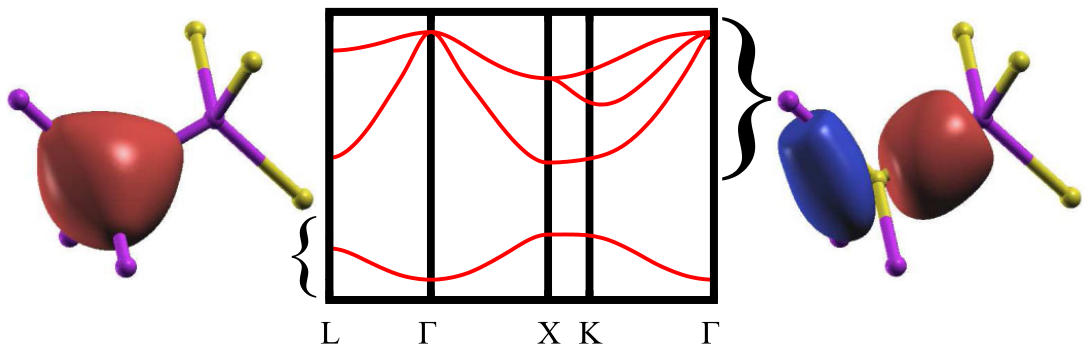
\includegraphics[scale=1.8]{GaAsps}{
\caption{\label{fig:2.2.2}
توابع وانییر بیشینه جایگزیده ساخته شده از نوار \lr{s} یا سه نوار \lr{p} در \lr{GaAs}\cite{Marzari2012}
}}
\end{figure}
 
 نمونه شکل \ref{fig:bloch} برای زمانی است که دو تصویر یا بیشتر کنار هم بخواهیم  است.
\begin{figure}[ht]
    \centering
    \begin{subfigure}[b]{0.4\textwidth}
        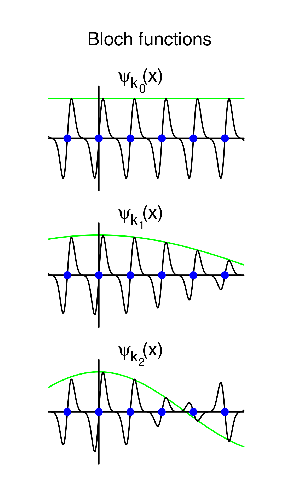
\includegraphics{bloch}
        \caption{شکل سمت راست}
        \label{fig:bloch}
    \end{subfigure}
    ~ %add desired spacing between images, e. g. ~, \quad, \qquad, \hfill etc. 
      %(or a blank line to force the subfigure onto a new line)
    \begin{subfigure}[b]{0.4\textwidth}
        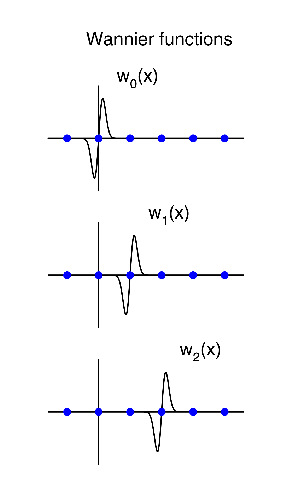
\includegraphics{wannier}
        \caption{شکل سمت چپ}
        \label{fig:wannier}
    \end{subfigure}
  \caption{
الف : توابع بلوخ متناظر با سه نقطه k مختلف در یک بعد در فضای واقعی که قسمت سبز رنگ، مربوط به پوش 
 $e^{i\mathbf{k}r}$
 است. ب : توابع وانیر جایگزیده که فضای متناظر با سمت چپ را تنیده است\cite{Marzari2012}}
\end{figure}

شکل نمونه زیر وقتی است که بخواهیم زیرنویس تصویر را کنارنویس کنیم در این صورت از بسته \lr{SCfigure} استفاده می کنیم.
\begin{SCfigure}
    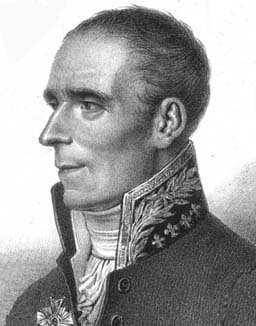
\includegraphics[width=0.35\textwidth]{Laplace}
        \caption{\protect\rule{0ex}{5ex}ایشان آقای لاپلاس است}
\end{SCfigure}
\newpage
%%%%%%%%%%%%%%%%%%%%%
\section{انواع لیست در\lr{LaTeX} }
در این بخش تلاش میگردد  انواع روش های ایجاد لیست در متن و نحوه استفاده از آنها بیان گردد. استفاده از لیست ها در 
\lr{\LaTeX}
بسیار راحت میباشد.   برای لیست هایی که نیاز به ترتیب خاص ندارند میتوان از محیط 
\lr{itemize} 
 و برای لیست های دارای ترتیب  میتوان از محیط
\lr{enumerate} 
استفاده کرد. استفاده از این دو محیط نیاز به افزودن بسته خاصی ندارد.
 برای ایجاد لیست بر اساس عنوان نیز میتوان از محیط 
\lr{decription}
استفاده کرد. لازم به ذکر است که برای استفاده از این محیط لازم است بسته
\lr{enumitem}
فراخوانی گردد.  


\subsection{لیست بدون ترتیب } 
 برای استفاده از محیط 
\lr{itemize}
 میتوان از دستور زیر استفاده نمود.
\begin{latin}
\begin{lstlisting}[style=Tex]
\begin{itemize}[label=$\ast$]
   \item %*\rl{یک}*)
   \item %*\rl{دو}*)
   \item %*\rl{سه}*)
\end{itemize}
\end{lstlisting}
\end{latin}

شایان ذکر است که آرگومان ورودی(در اینجا 
\verb![label=$\ast$]!
)
 شکل مورد استفاده برای لیست بندی را مشخص میکند.این دستور خروجی به شکل زیر ایجاد میکند.
\begin{itemize}[label=$\ast$]
\item یک
\item دو
\item سه
\end{itemize}
در صورتی که نیاز باشد نمادهای مورد استفاده در لیست تغییر کنند، میتوان بصورت زیر نمادها را تغییر داد.
\begin{latin}
\begin{lstlisting}[style=Tex]
\begin{itemize}
   \item[$-$] %*\rl{دش\hspace{2 em}}*)
   \item[$\ast$] %*\rl{ستاره}*)
   \item[$+$] %*\rl{پلاس\hspace{2 em}}*)
\end{itemize}
\end{lstlisting}
\end{latin}
که نتیجه خروجی به شکل زیر میباشد:
\begin{itemize}
    \item[$-$] دش
    \item[$\ast$] ستاره
    \item[$+$] پلاس
\end{itemize}



\subsection{لیست های دارای ترتیب }
برای ایجاد لیست دارای ترتیب میتوان از محیط 
\lr{enumerate} 
به شکل زیر استفاده نمود.
\begin{latin}
 \begin{lstlisting}[style=Tex]
\begin{enumerate}[label=\alph*)]
   \item %*\rl{یک}*)
   \item  %*\rl{دو}*)
   \item  %*\rl{سه}*)
\end{enumerate}
\end{lstlisting}
\end{latin}
 
آرگومان ورودی 
\verb![label=\alph*)]!
شیوه ترتیب بندی را مشخص میکند. میتوان از دستور 
\verb![label=(\roman*)]!
برای شماره گذاری با حروف یونانی و از دستور 
\verb![label=\arabic*)]!
برای شماره گذاری با اعداد فارسی استفاده نمود.
خروجی این دستور به شکل زیر میباشد.

\begin{enumerate}[label=\alph*)]
	\item یک
	\item دو
	\item سه
\end{enumerate}



در صورتی که در ایجاد لیست نیاز به زیرگروه نیز باشد. میتوان به شکل زیر این زیرگروهها را ایجاد کرد:


\begin{latin}
\begin{lstlisting}[style=Tex]
\begin{enumerate}[label=(\roman*)]
    \item  %*\rl{یک}*)
    \begin{enumerate}[label=(\arabic*)]
        \item  %*\rl{دو}*)
        \item  %*\rl{سه}*)
        \item  %*\rl{چهار}*)
    \end{enumerate}
    \item  %*\rl{پنج}*)
    \item  %*\rl{شش}*)
\end{enumerate}
\end{lstlisting}
\end{latin}
 که نتیجه خروجی آن به شکل زیر میباشد:

\begin{enumerate}[label=(\roman*)]
	\item یک 
    \begin{enumerate}[label=(\arabic*)]
    	\item دو
        \item سه
        \item چهار
    \end{enumerate}
    \item پنج
    \item شش
\end{enumerate}

\subsection{ایجاد لیست با عنوان دلخواه } 
برای اینکه از عناوین در ایجاد لیست استفاده شود می توان از محیط 
\lr{description}
 به صورت زیر استفاده نمود.
\begin{latin}
\begin{lstlisting}[style=Tex]
\begin{description}
   \item[Biology] %*\rl{زیست شناسی\hspace{2 em}}*) 
   \item[Physics] %*\rl{علم فیزیک\hspace{2 em}}*) 
   \item[Psychology] %*\rl{روانشناسی}*) 
\end{description}
\end{lstlisting}
\end{latin}
که نتیجه خروجی به صورت زیر میباشد:
\begin{description}
\item[Biology]  زیست شناسی
\item[Physics] علم مواد و حرکت
\item[Psychology] روانشناسی
\end{description}
%%%%%%%%%%%%%%%%%%%%5
\section{نوشتن جداول}\label{seq:3.4}
رای رسم جدول در لاتک از \lr{tabular} استفاده می‌شود. نخست باید آغاز و پایان آن را مشخص کنیم.
\begin{latin}
\begin{lstlisting}[style=Tex]
\begin{tabular}{lcr}

\end{tabular}
\end{lstlisting}
\end{latin}

هم‌زمان با این کار باید تعداد ستون‌های جدول نیز به لاتک معرفی شود. این کار با افزودن یکی از حروف c (برای ستونی با داده‌های مرکزچین)، l (برای ستونی با داده‌های چپ چین) و r (برای ستونی با داده‌های راست‌چین) داخل آکلاد انجام می‌شود، یعنی برای یک ستون راست‌چین از یک r، دو ستون راست‌چین دو r و .... سپس داده‌های سطر اول را در بین شروع و پایان محیط \lr{tabular} قرار می‌دهیم. برای رفتن به سطر بعد هم از\textbackslash\textbackslash استفاده می‌کنیم.

محیط \lr{tabular} نیز مثل یک قسمت از متن تلقی می‌شود و برای اینکه خصوصیات یک محیط پویا(شناور) را به آن بدهیم آن را در محیط \lr{table} قرار داده و از دستور مربوطه برای وسط چین کردن و دادن عنوان هم بهره خواهیم برد(همانند محیط \lr{figure} پارامترهای اختیاری مربوط به \lr{table} هم به صورت کاملا مشابه قابل تنظیم هستند).

\begin{latin}
\begin{lstlisting}[style=Tex]
\begin{table}[htbp]
\centering
\caption{title}
\begin{tabular}{lcr}
column1 & column2 & column3 \\
column1 & column2 & column3 \\
column1 & column2 & column3 \\
\end{tabular}
\end{table}
\end{lstlisting}
\end{latin}
%%%%%%%%%
\section{قالب دهی به جدول و تعریف آن به صورت شناور}

برای رسم خطوط جدا کننده در بین ستون ها یا سطرها از فرمان ها و نکات زیر استفاده می‌کنیم:
\begin{itemize}
\item  اگر به هنگام تعریف محیط \lr{tabular} در آرگومان دوم بین ستون ها از کاراکتر \textbar (پایپ) استفاده کنید، به همان ترتیب و به همان تعداد بین ستون ها خط ایجاد می‌شود.
\item برای تعریف خطوط بین سطرها باید در مکان مناسب از فرمان \lr{$\backslash$hline} استفاده کنید. به تعداد دلخواه می‌توانید از این فرمان استفاده نمایید.
\item اگر می‌خواهید در پایان جدول نیز خط افقی رسم کنید، برخلاف گفته قبلی این بار باید در انتهای سطر آخر نیز از کاراکترهای \textbackslash\textbackslash استفاده نمایید.
\item  اگر می‌خواهید به جای رسم یک خط کامل بین سطرهای جدول، از خطوط ناقص استفاده کنید، باید از فرمان زیر استفاده کنید:
\end{itemize}

\begin{latin}
\begin{lstlisting}[style=Tex]
\cline{column#1 – column#N}
\end{lstlisting}
\end{latin}

\section{تعریف جدول به صورت شناور و نحوه ارجاع دادن به آن}
برای تعریف جدول به صورت شناور و همچنین قابلیت ارجاع دهی و \lr{caption} گذاری، باید به جدول به عنوان یک موجودیت مستقل نگاه کنید. برای اینکار باید آنرا در داخل یک محیط دیگر بنام محیط \lr{table} تعریف کنید.
\begin{latin}
\begin{lstlisting}[style=Tex]
\begin{table}
\begin{tabular}
...
\end{tabular}
\end{table}
\end{lstlisting}
\end{latin}

\noindent
\textbf{
نکته ۱} : محیط \lr{table} نیز همانند محیط \lr{figure} از محیط های شناور است و خود لاتکس در مورد محل قرارگیری آن در صفحه تصمیم می‌گیرد.\\
\textbf{نکته ۲} : با استفاده از دستور

\begin{latin}
\begin{lstlisting}[style=Tex]
\caption {name}
\end{lstlisting}
\end{latin}

می‌توان به جدول زیرنویس اختصاص داد.\\
\textbf{نکته ۳: }برای ارجاع دادن به یک جدول همانند تصویر، ابتدا باید یک \lr{lable} به آن اختصاص دهید و در ادامه با استفاده از \lr{lable} به آن ارجاع دهید.

در زیر یک نمونه از جدول آمده است.
\begin{latin}
 \begin{lstlisting}[style=Tex]
 \begin{table}[ht]
\begin{center}
\caption{ %*\rl{
انتخاب‌های مختلف برای قسمت شعاعی توابع حدس اوّلیّه،}*)
$\alpha=Z/a$ \cite{Wannier902013}. \label{tab:radial2}}
\begin{latin}
\renewcommand{\arraystretch}{0.6}
\begin{tabular}{|cc|}
\hline
 $n$ & $R_{\mathrm{n}}({\bf r})$ \\\hline
1        &  $2 \alpha^{3/2}\exp(-\alpha r)$ \\\hline
2        &  $\frac{1}{2\sqrt{2}}\alpha^{3/2}(2-\alpha r)\exp(-\alpha r/2)$ \\\hline
3        &  $\sqrt{\frac{4}{27}}\alpha^{3/2}(1-2\alpha r/3+2\alpha^{2}r^{2}/27)\exp(-\alpha r/3)$ \\\hline
\end{tabular}
\end{latin}
\end{center}
\end{table}  
 \end{lstlisting}

\end{latin}
که خروجی به شکل زیر دارد
\begin{table}[ht]
\begin{center}
\caption{ 
انتخاب‌های مختلف برای قسمت شعاعی توابع حدس اوّلیّه،
$\alpha=Z/a$ \cite{Wannier902013}. \label{tab:radial2}}
\begin{latin}
\renewcommand{\arraystretch}{0.6}
\begin{tabular}{|cc|}
\hline
 $n$ & $R_{\mathrm{n}}({\bf r})$ \\\hline
1        &  $2 \alpha^{3/2}\exp(-\alpha r)$ \\\hline
2        &  $\frac{1}{2\sqrt{2}}\alpha^{3/2}(2-\alpha r)\exp(-\alpha r/2)$ \\\hline
3        &  $\sqrt{\frac{4}{27}}\alpha^{3/2}(1-2\alpha r/3+2\alpha^{2}r^{2}/27)\exp(-\alpha r/3)$ \\\hline
\end{tabular}
\end{latin}
\end{center}
\end{table}

همانطور که مشاهده می‌شود خانه‌های جدول با \& و سطور با استفاده از \textbackslash\textbackslash از هم جدا می شوند و \lr{\textbackslash{hline}} برای ایجاد خط فاصل بین سطور استفاده می‌شود. سایر ساختار در جداول مشابه به تصاویر است.
\begin{table}[h]
\begin{center}
\renewcommand{\arraystretch}{0.6}
\begin{latin}
\begin{tabular}{|c|c|c|c|}
\hline
$l$ & $m_{\mathrm{r}}$ & Name & $\Theta_{lm_{\mathrm{r}}}(\theta,\varphi)$ \\\hline
 0  &  1  &  \verb#s#   & $\frac{1}{\sqrt{4\pi}}$ \\\hline
 1  &  1  &  \verb#pz#  & $\sqrt{\frac{3}{4\pi}}\cos\theta$ \\\hline
 1  &  2  &  \verb#px#  & $\sqrt{\frac{3}{4\pi}}\sin\theta\cos\varphi$ \\\hline
 1  &  3  &  \verb#py#  & $\sqrt{\frac{3}{4\pi}}\sin\theta\sin\varphi$ \\\hline
 2  &  1  &  \verb#dz2# &$\sqrt{\frac{5}{16\pi}}(3\cos^{2}\theta -1)$ \\\hline
 2  &  2  &  \verb#dxz# & $\sqrt{\frac{15}{4\pi}}\sin\theta\cos\theta\cos\varphi$ \\\hline
 2  &  3  &  \verb#dyz# &$\sqrt{\frac{15}{4\pi}}\sin\theta\cos\theta\sin\varphi$ \\\hline
 2  &  4  &  \verb#dx2-y2# &$\sqrt{\frac{15}{16\pi}}\sin^{2}\theta\cos2\varphi$ \\\hline
 3  &  6  &  \verb#fx(x2-3y2)# & $\frac{\sqrt{35}}{4\sqrt{2\pi}}\sin^{3}\theta(\cos^{2}\varphi-3\sin^{2}\varphi)\cos\varphi$\\\hline
 3  &  7  &  \verb#fy(3x2-y2)# & $\frac{\sqrt{35}}{4\sqrt{2\pi}}\sin^{3}\theta(3\cos^{2}\varphi-\sin^{2}\varphi)\sin\varphi$\\\hline
\end{tabular}
\end{latin}
\caption{توابع زاویه‌ای}
\label{tab:angular}
\end{center}
\end{table}

نمونه زیر یک جدول فارسی است
\begin{table}[h]
\begin{center}
 \begin{tabular}
    {>{\columncolor{blue}\color{white}\bfseries}rl}
\rowcolor[gray]{0.8}
    \color{black} روز & \bfseries تعداد حاضرین\\[2pt]
دوشنبه&    57 \\  سشنبه&   11 \\
چهرشنبه& 96 \\  پنجشنبه& 122 \\
جمعه&   210 \\  شنبه& 198 \\
یکشنبه&    40 \\
\cellcolor[gray]{0.8}\color{black}جمع& 724
\end{tabular}
\caption{نمونه‌ای دیگر از جدول}
 \end{center}
\end{table}


%چنانچه بسته  float  را استفاده کنید بایستی از دستورات زیر برای تغییر در caption جداول استفاده کنید که در این صورت با فعالسازی دستور زیر از این به بعد جداول با caption  در بالا خواهند آمد. به توضیحات فایل main رجوع کنید
% \floatsetup[table]{capposition=bottom}
% \floatsetup[table]{capposition=top}

جدول به صورت لندسکیپ
 \begin{landscape}
\begin{table}[h]
\begin{center}
\caption{ انتخاب‌های مختلف برای قسمت شعاعی توابع حدس اوّلیّه،$\alpha=Z/a$ \cite{Wannier902013}. \label{tab:radial}}
\begin{latin}
\renewcommand{\arraystretch}{0.6}
\begin{tabular}{|cc|}
\hline\hline
&\\
\ \ $n$ \ \ & $R_{\mathrm{n}}({\bf r})$ \\
&\\\hline&\\
1        &  $2 \alpha^{3/2}\exp(-\alpha r)$ \\
&\\\hline&\\
2        &  $\frac{1}{2\sqrt{2}}\alpha^{3/2}(2-\alpha
r)\exp(-\alpha r/2)$ \\
&\\\hline&\\
3        &  $\sqrt{\frac{4}{27}}\alpha^{3/2}(1-2\alpha r/3+2\alpha^{2}r^{2}/27)\exp(-\alpha r/3)$ \\
&\\\hline\hline
\end{tabular}
\end{latin}
\end{center}
\end{table}
\end{landscape}
%%%%%%%%%%%%%%%%%%%%%%%%%%%%%%%%%%%%
 \section{محیط های ریاضی}
 می توانید از محیط های زیر استفاده کنید
 
 \begin{tabular}{|c|c|}
\hline
definition&section\\\hline
theorem & قضیه\\\hline
lemma&لم\\\hline
proposition&گزاره\\\hline
corollary&نتیجه\\\hline
remark&ملاحظه\\\hline
example&مثال\\\hline
\hline
 \end{tabular}
\subsection{ قضیه انتخاب}
در این قسمت نشان می دهیم
\begin{lemma}\textbf{(قطری سازی)}
نمونه یک لم اینجا آمده است.
\end{lemma}
\begin{proof}
نمونه یک اثبات  در اینجا آمده است.
\end{proof}
\begin{remark}
اگر به ازای تمام مقادیر n داشته باشیم
$|u_n(.)|\leqslant M$
\end{remark}
\begin{theorem}
نمونه ای دیگر
\end{theorem}
\begin{example}
 نمونه مثال
\end{example}
%%%%%%%%%%%%%%%%%%%%%%%
\section{\lr{tikz} و استفاده از آن}

بسته تیکز (\lr{Tikz}) احتمالاً قدرتمندترین ابزار برای تولید اشکال گرافیکی در لاتک است. به منظور استفاده از آن ابتدا باید قابلیت تصویرپردازی تیکز را با قرار دادن دستور زیر در دیباچه (\lr{preamble}) فایل متنی فعال کنید:
\begin{latin} 
\begin{lstlisting}
\usepackage{tikz}
\end{lstlisting}
\end{latin} 
محیط تصویرپردازی تیکز در متن با قرار دادن دستورات \lr{\textbackslash{begin\{tikzpicture}\}} و \lr{\textbackslash{end\{tikzpicture}\}} به ترتیب در ابتدا و انتهای دستورات این محیط فعال می‌شود. به عنوان مثال یک شکل گرافیکی را می‌توان به سادگی با تعدادی دستور مطابق زیر تولید کرد:
\begin{latin} 
\begin{lstlisting}[style=Tex]
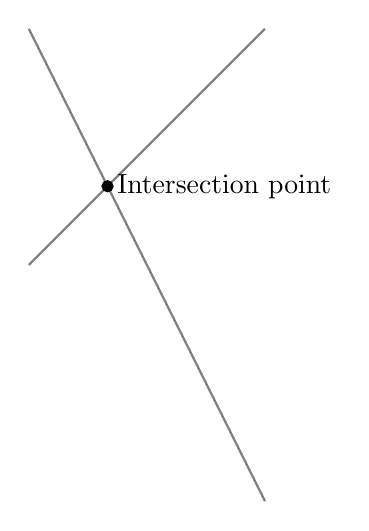
\begin{tikzpicture}
\draw[gray, thick] (-1,2) -- (2,-4);
\draw[gray, thick] (-1,-1) -- (2,2);
\filldraw[black] (0,0) circle (2pt) node[anchor=west] {Intersection point};
\end{tikzpicture}
\end{lstlisting}
\end{latin} 

خروجی این دستورات به شکل زیر است:

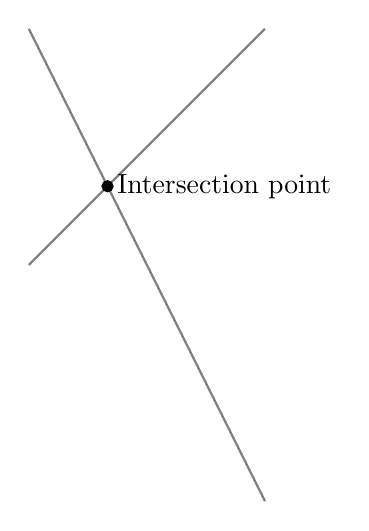
\begin{tikzpicture}
\draw[gray, thick] (-1,2) -- (2,-4);
\draw[gray, thick] (-1,-1) -- (2,2);
\filldraw[black] (0,0) circle (2pt) node[anchor=west] {Intersection point};
\end{tikzpicture}

در این مثال دو خط و یک نقطه رسم شده است. به منظور تولید خط از دستور \lr{\textbackslash{draw[gray, thick]}} استفاده شده که در آن یک المان گرافیکی تعریف شده که رنگ آن خاکستری (\lr{gray}) و ضخامت آن کلفت (\lr{thick}) است. خط در حقیقت با استفاده از دو نقطه انتهایی آن \lr{(-1,2)} و \lr{(2,-4)} که با علامت \lr{--} به هم متصل شده اند تعریف شده است. نقطه نیز در واقع یک دایره توپر است که با استفاده از دستور \lr{\textbackslash{filldraw[black]}} رسم شده است. در این دستور مرکز دایره نقطه \lr{(0,0)} و شعاع آن \lr{(2pt)} تعیین شده است. در جلوی آن یک گره (\lr{node}) تعریف شده که در حقیقت یک جعبه می‌باشد که شامل یک متن (در اینجا متن \lr{"intersection point"}) است که با دستور \lr{[anchor=west]} در سمت راست نقطه قرار داده شده است. توجه کنید که در انتهای هر دستور رسم باید علامت نقطه ویرگول (\lr{;}) را قرار دهید.

توجه: محیط رسم شکل تیکز را می‌توان در یک محیط دیگر مانند محیط شکل (\lr{figure}) قرار داد. 

شکلهای زیاد و با گرافیک بالایی را می توان با استفاده از \lr{tikz} تولید نمود .
%%%%%%%%%%%%%%%%%%%%%%%%%%%%%%%
\usetikzlibrary{lindenmayersystems}

\pgfdeclarelindenmayersystem{A}{
    \rule{F -> FF[+F][-F]}
}

\pgfdeclarelindenmayersystem{B}{
    \rule{F -> ffF[++FF][--FF]}
}

\pgfdeclarelindenmayersystem{C}{
    \symbol{G}{\pgflsystemdrawforward}
    \rule{F -> F[+F][-F]FG[+F][-F]FG}
}

\pgfdeclarelindenmayersystem{D}{
    \symbol{G}{\pgflsystemdrawforward}
    \symbol{H}{\pgflsystemdrawforward}
    \rule{F -> H[+HG][-HG]G}
    \rule{G -> HF}
}

\tikzset{
    type/.style={l-system={#1, axiom=F,order=3,step=4pt,angle=60},
      blue, opacity=0.4, line width=.5mm, line cap=round   
    },
}

\newcommand\drawsnowflake[2][scale=0.2]{
    \tikz[#1]
    \foreach \a in {0,60,...,300}  {
    \draw[rotate=\a,#2] l-system;
    };
}

\begin{center}
\foreach \width in {.2,.4,...,.8} 
{  \drawsnowflake[scale=0.3]{type=A, line width=\width mm} }

\foreach \width in {.2,.4,...,.8} 
{  \drawsnowflake[scale=0.38]{type=A, l-system={angle=90}, line width=\width mm} }    

\foreach \width in {.2,.4,...,.8} 
{  \drawsnowflake[scale=0.3]{type=B, line width=\width mm} }

\foreach \width in {.2,.4,...,.8} 
{  \drawsnowflake{type=B, l-system={angle=30}, line width=\width mm} }

\drawsnowflake[scale=0.24]{type=C, l-system={order=2}, line width=0.2mm}
\drawsnowflake[scale=0.25]{type=C, l-system={order=2}, line width=0.4mm}
\drawsnowflake[scale=0.25]{type=C, l-system={order=2,axiom=fF}, line width=0.2mm}
\drawsnowflake[scale=0.32]{type=C, l-system={order=2,axiom=---fff+++F}, line width=0.2mm}

\drawsnowflake[scale=0.38]{type=D, l-system={order=4,angle=60,axiom=GF}, line width=0.7mm}
\drawsnowflake[scale=0.38]{type=D, l-system={order=4,angle=60,axiom=GfF}, line width=0.7mm}
\drawsnowflake[scale=0.38]{type=D, l-system={order=4,angle=60,axiom=FG}, line width=0.7mm}
\drawsnowflake[scale=0.38]{type=D, l-system={order=4,angle=60,axiom=FfG}, line width=0.7mm}
\end{center}
%%%%%%%%%%%%%%%%%%%
در آدرس زیر نمونه‌های بیشتر را ببینید.
\begin{latin}
 \url{http://www.texample.net/tikz/examples/}
\end{latin}
نمونه‌ای از فلوچارت در ادامه آمده است
\begin{figure}[h!]
 \begin{center}
  \tikzstyle{startstop} = [rectangle, rounded corners, minimum width=3cm,text width=13.5em, minimum height=1cm,text badly centered, draw, fill=red!30]
  \tikzstyle{io} = [trapezium, trapezium left angle=70, trapezium right angle=110, minimum width=3cm, minimum height=1cm, text centered, draw, fill=blue!30]
  \tikzstyle{process} = [rectangle, minimum width=3cm, minimum height=1cm, text centered, draw=black, fill=orange!30]
  \tikzstyle{arrow} = [thick,->,>=stealth]
   \tikzstyle{decision} = [diamond, draw, fill=green!30,text width=4.5em, text badly centered, node distance=3cm, inner sep=0pt]
  \tikzstyle{block} = [rectangle, draw, fill=blue!20,text width=5em, text centered, rounded corners, minimum height=4em]
  \tikzstyle{line} = [draw, -latex']
  \tikzstyle{cloud} = [draw, ellipse,fill=red!20, node distance=3cm,minimum height=2em]
  \begin{tikzpicture}[node distance=2.1cm,auto]
  \node (start) [startstop] {\rl{دریافت توابع موج بلوخ از کد ساختار الکترونی و شروع فرآیند کمینه سازی}};
  \node (pro1) [process,below of=start] {$|\phi_{n\bf k}\rangle=\sum_{m}|\psi_{m\bf k}\rangle\langle\psi_{m\bf k}|g_n\rangle$};
  \node (pro2) [process,below of=pro1] {$S_{mn}^{({\bf k})}=\langle\phi_{m\bf k}|\phi_{n\bf k}\rangle=\left(A^\dagger A\right)_{mn}$};
  \node (pro3) [process,below of=pro2] {$|\tilde{\phi}_{n\bf k}\rangle=\sum_{m}\left(S^{-1/2}\right)_{mn}|\phi_{m\bf k}\rangle$};
  \node (pro4) [process,left of=start,xshift=-7cm] {$u_{n\bf k}^{(0)}({\bf k})=\exp{(-i{\bf k.r})}\tilde{\phi}_{m\bf k}({\bf r})$};
  \node (pro5) [process,below of=pro4] {$M_{mn}^{(0)({\bf k,b})}=\langle u_{m \bf k}^{(0)}|u_{m \bf k+b}^{(0)}\rangle$};
  \node (pro6) [process,below of=pro5] {$U_{mn}^{({\bf k})}=AS^{-\frac{1}{2}}$};
   \node (pro7) [process,below of=pro6] {$G^{({\bf k})}=\frac{d\Omega}{dW^{({\bf k})}}=f(M_{mn}^{\bf k,b})$};
  \node (dec1) [decision, below of=pro7] {$G^{({\bf k})}=0$};
  \node (pro8) [process,below of=dec1,yshift=-1cm] {$\Delta W^{({\bf k})}=\epsilon G^{({\bf k})}$};
  \node (pro9) [process,below of=pro8] {$U_{new}^{({\bf k})} \rightarrow U_{old}^{({\bf k})} \exp{[\Delta W^{({\bf k})}]}$};
  \node(pro10)[process,below of=pro9]{$ M^{({\bf k,b})}=U^{({\bf k})\dagger}M^{(0)({\bf k,b})}U^{({\bf k,b})}$};
  \node(result)[io,right of=dec1,xshift=6cm,yshift=-3cm]{$w_{n{\bf R}}({\bf r})=\frac{V}{(2\pi)^3}\int_{\mathrm{BZ}}\left[\sum_{m} U^{({\bf k})}_{mn} \psi_{m{\bf k}}({\bf r})\right]e^{-\mathrm{i}{\bf k}.{\bf R}} \:\mathrm{d}{\bf k}$};
  \node (end) [startstop,below of=result,yshift=-0.5cm] {\rl{پایان}};
  \draw[arrow] (start) -- (pro1);
  \draw [arrow] (pro1) -- (pro2);
  \draw [arrow] (pro2) -- (pro3);
  \draw [arrow] (pro3.west) -- node[anchor=north]{}+(-3cm,0)|-(pro4);
  \draw [arrow] (pro4)--(pro5);
  \draw [arrow] (pro5)--(pro6);
  \draw [arrow] (pro6)--(pro7);
  \draw [arrow] (pro7)--(dec1);
  \draw [arrow] (dec1.east) -- node[anchor=south]{\rl{بله}}+(7,0)-| (result);
  \draw[arrow] (dec1.south) -- node[anchor=west]{\rl{خیر}}+(0,-1)--(pro8);
  \draw[arrow] (pro8)--(pro9);
  \draw[arrow] (pro9)--(pro10);
  \draw[arrow](pro10.west)-- node[]{}+(-0.5cm,0)|-(dec1.west);
  \draw[arrow] (result)--(end);
  \end{tikzpicture}
 \end{center}
\caption{روندنمای محاسبه‌ی توابع وانییر بیشینه جایگزیده}\label{fig:3.8.1}
\end{figure}
برای دیدن چگونگی تولید روند نمای بالا با استفاده از \lr{Tikz} به کد منبع پایان‌نامه رجوع کنید.
